\subsubsection{Begreper}
Her er noen begreper som brukes om pulstog:
\\\\
Periodetid $T$: avstand fra bynelsen av en puls til bynelsen av neste. \\
PulseWidth $PW$: avstand fra bynelse til slutt av en puls. \\
DutyCycle (i prosent): $\frac{PW}{T} \cdot 100$
\\\\
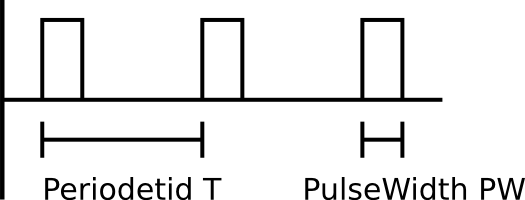
\includegraphics[width=0.5\textwidth]{./img/pulstog}

\paragraph{Uperfekt virkelighet} \mbox{} \\
Firkantbølgen stiger ikke momentant.\\
Amplitude: høyeste variasjon i spenning. \\
PulseWidth: Avstand fra første $50\%$ til neste. \\
Flanker: Stigning og nedgang. \\
Rise time: Tid fra $10\%$ opp til $90\%$. \\
Fall time: motsatt av rise time.
\\\\
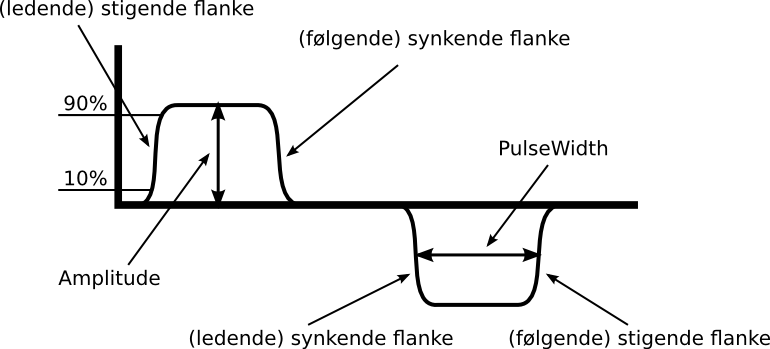
\includegraphics[width=\textwidth]{./img/pulstog2}



\subsubsection{Firkantbølge fra sinusbølger}
Ved å generere to sinusbølger
kan man addere dem sammen for å tilnærme en firkantbølge.
\\
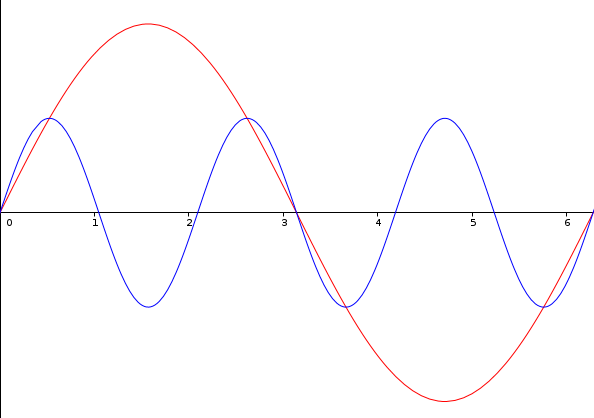
\includegraphics[width=\textwidth]{./img/harmoni-ab}
Vi har to funksjoner: \\
{\color{red} $a = 2\sin{x}$} \\
{\color{blue} $b = \sin{3x}$}
\\
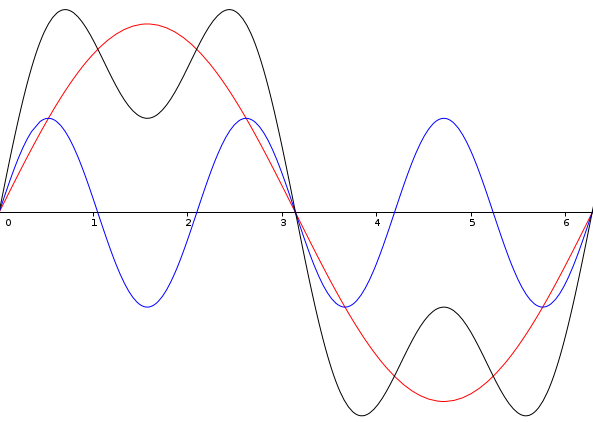
\includegraphics[width=\textwidth]{./img/harmoni-abc}
Lagt sammen blir \\
$c = $ {\color{red} $a$} $+$ {\color{blue} $b$} \\
Du kan se at det begynner å ligne på en firkantbølge.
\\\\
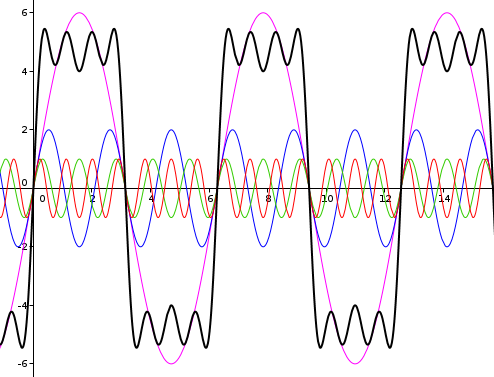
\includegraphics[width=\textwidth]{./img/harmoni-1357}
Her er et eksempel med 1, 3, 5 og 7 harmoni.
